\section{Durchführung}
\label{sec:Durchführung}
\begin{figure}
  \centering
  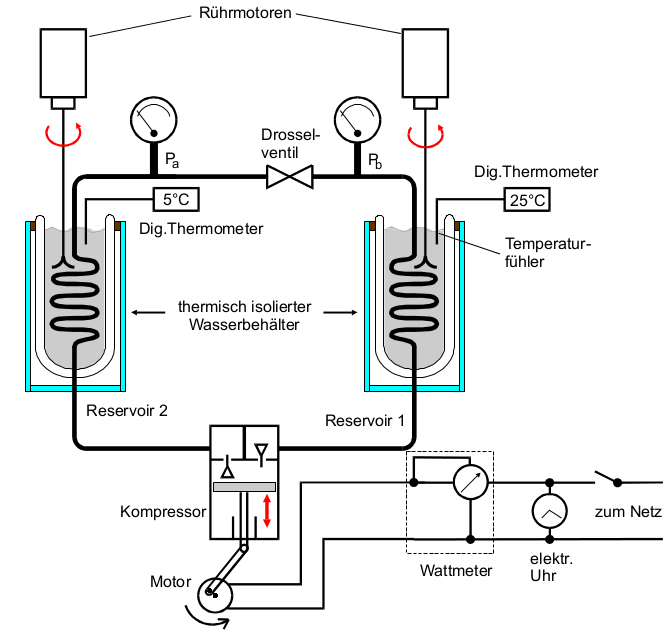
\includegraphics[width=0.60\textwidth]{messapparatur.png}
  \caption{Aufbau der Messapparatur\cite{sample}.}
  \label{fig:aufbau}
\end{figure}
Zu Beginn werden die Reservoire 1 und 2 mit Wasser gefüllt. Um die Menge genau
messen zu können wird ein Messkolben verwendet.
Es werden der Kompressor und die Rührmotoren, die dafür sorgen, dass die Temperatur in
den Behältern immer gleichmäßig verteilt ist, angeschaltet.
Nun werden in festen Zeitabständen die Temperaturen $T_1$ und $T_2$, die Drücke
$p_\symup{a}$ und $p_\symup{b}$, sowie die Leistungsaufnhame $N$ des Kompressors
abgelesen. Dies wird solange wiederholt, bis die Temperatur $T_1$ 320,15\si{\kelvin}
erreicht hat. Da die Manometer bei Umgebungsdruck auf 0 Bar geeicht sind,
muss auf alle abgelesenen Drücke 1 Bar addiert werden.
